\chapter{Задача слежения для системы с астатизмом нулевого порядка (П-регулятор)}
Создадим единую схему Simulink для Задачи 3 - 5 с помощью блоков Multiport Switch:
\begin{figure}[H]
    \centering
    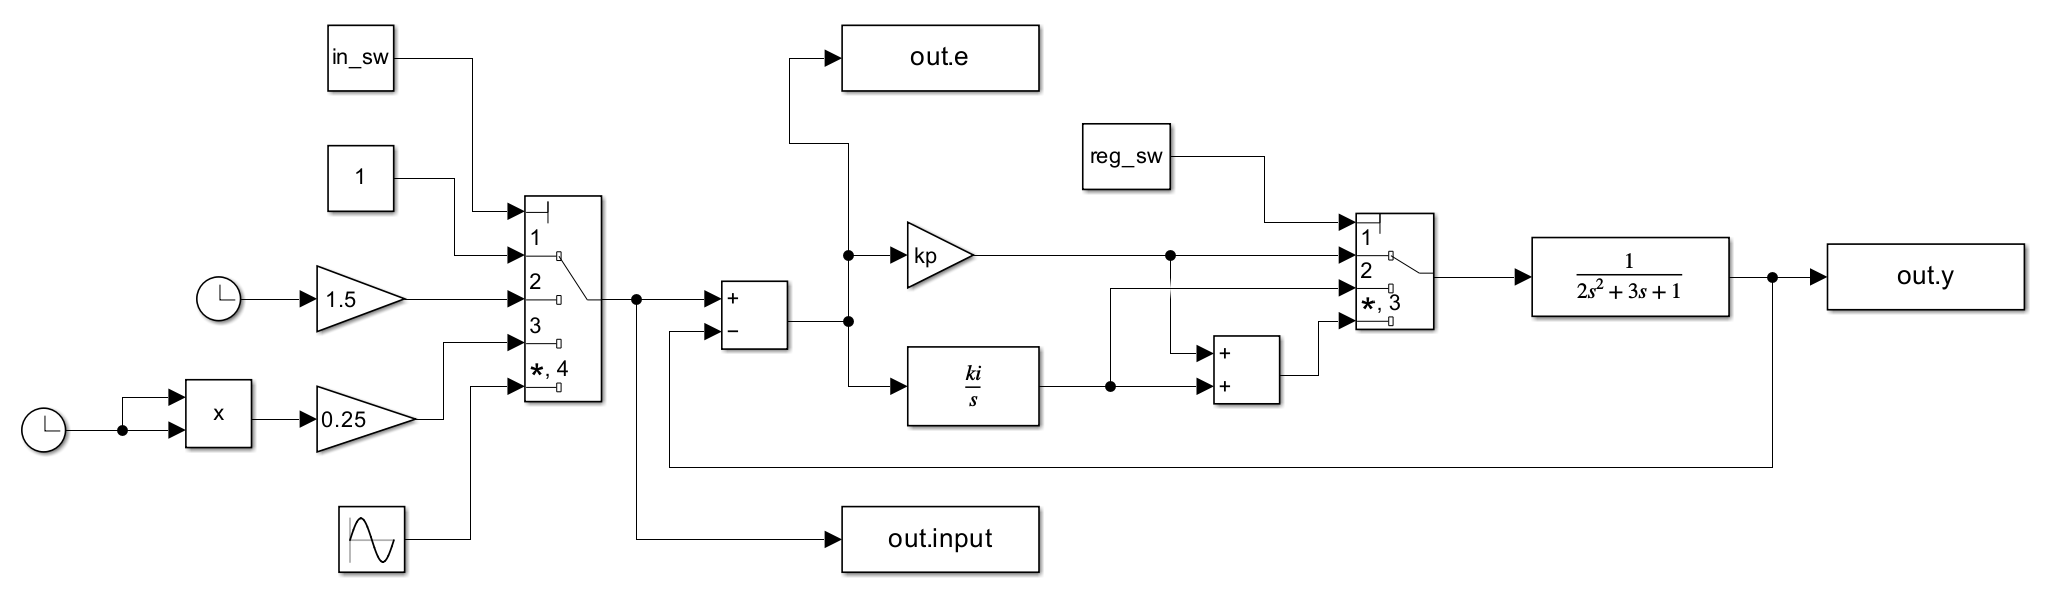
\includegraphics[width=1\textwidth, trim={1cm 0cm 1cm 0cm}]{../images/sim4.png}
    \caption{Схема замкнутой системы с П, И, ПИ регуляторами в Simulink}
    \label{fig:sim4}
\end{figure}

Зададимся следующими параметрами $k_p$:
\begin{enumerate}
    \item $k_p = 1$
    \item $k_p = 10$ 
    \item $k_p = 100$
\end{enumerate}
\newpage
\section{Стационарный режим $g(t) = A$}
Выполним моделирование:
\begin{figure}[H]
    \centering
    \begin{minipage}{0.45\textwidth}
        \centering
        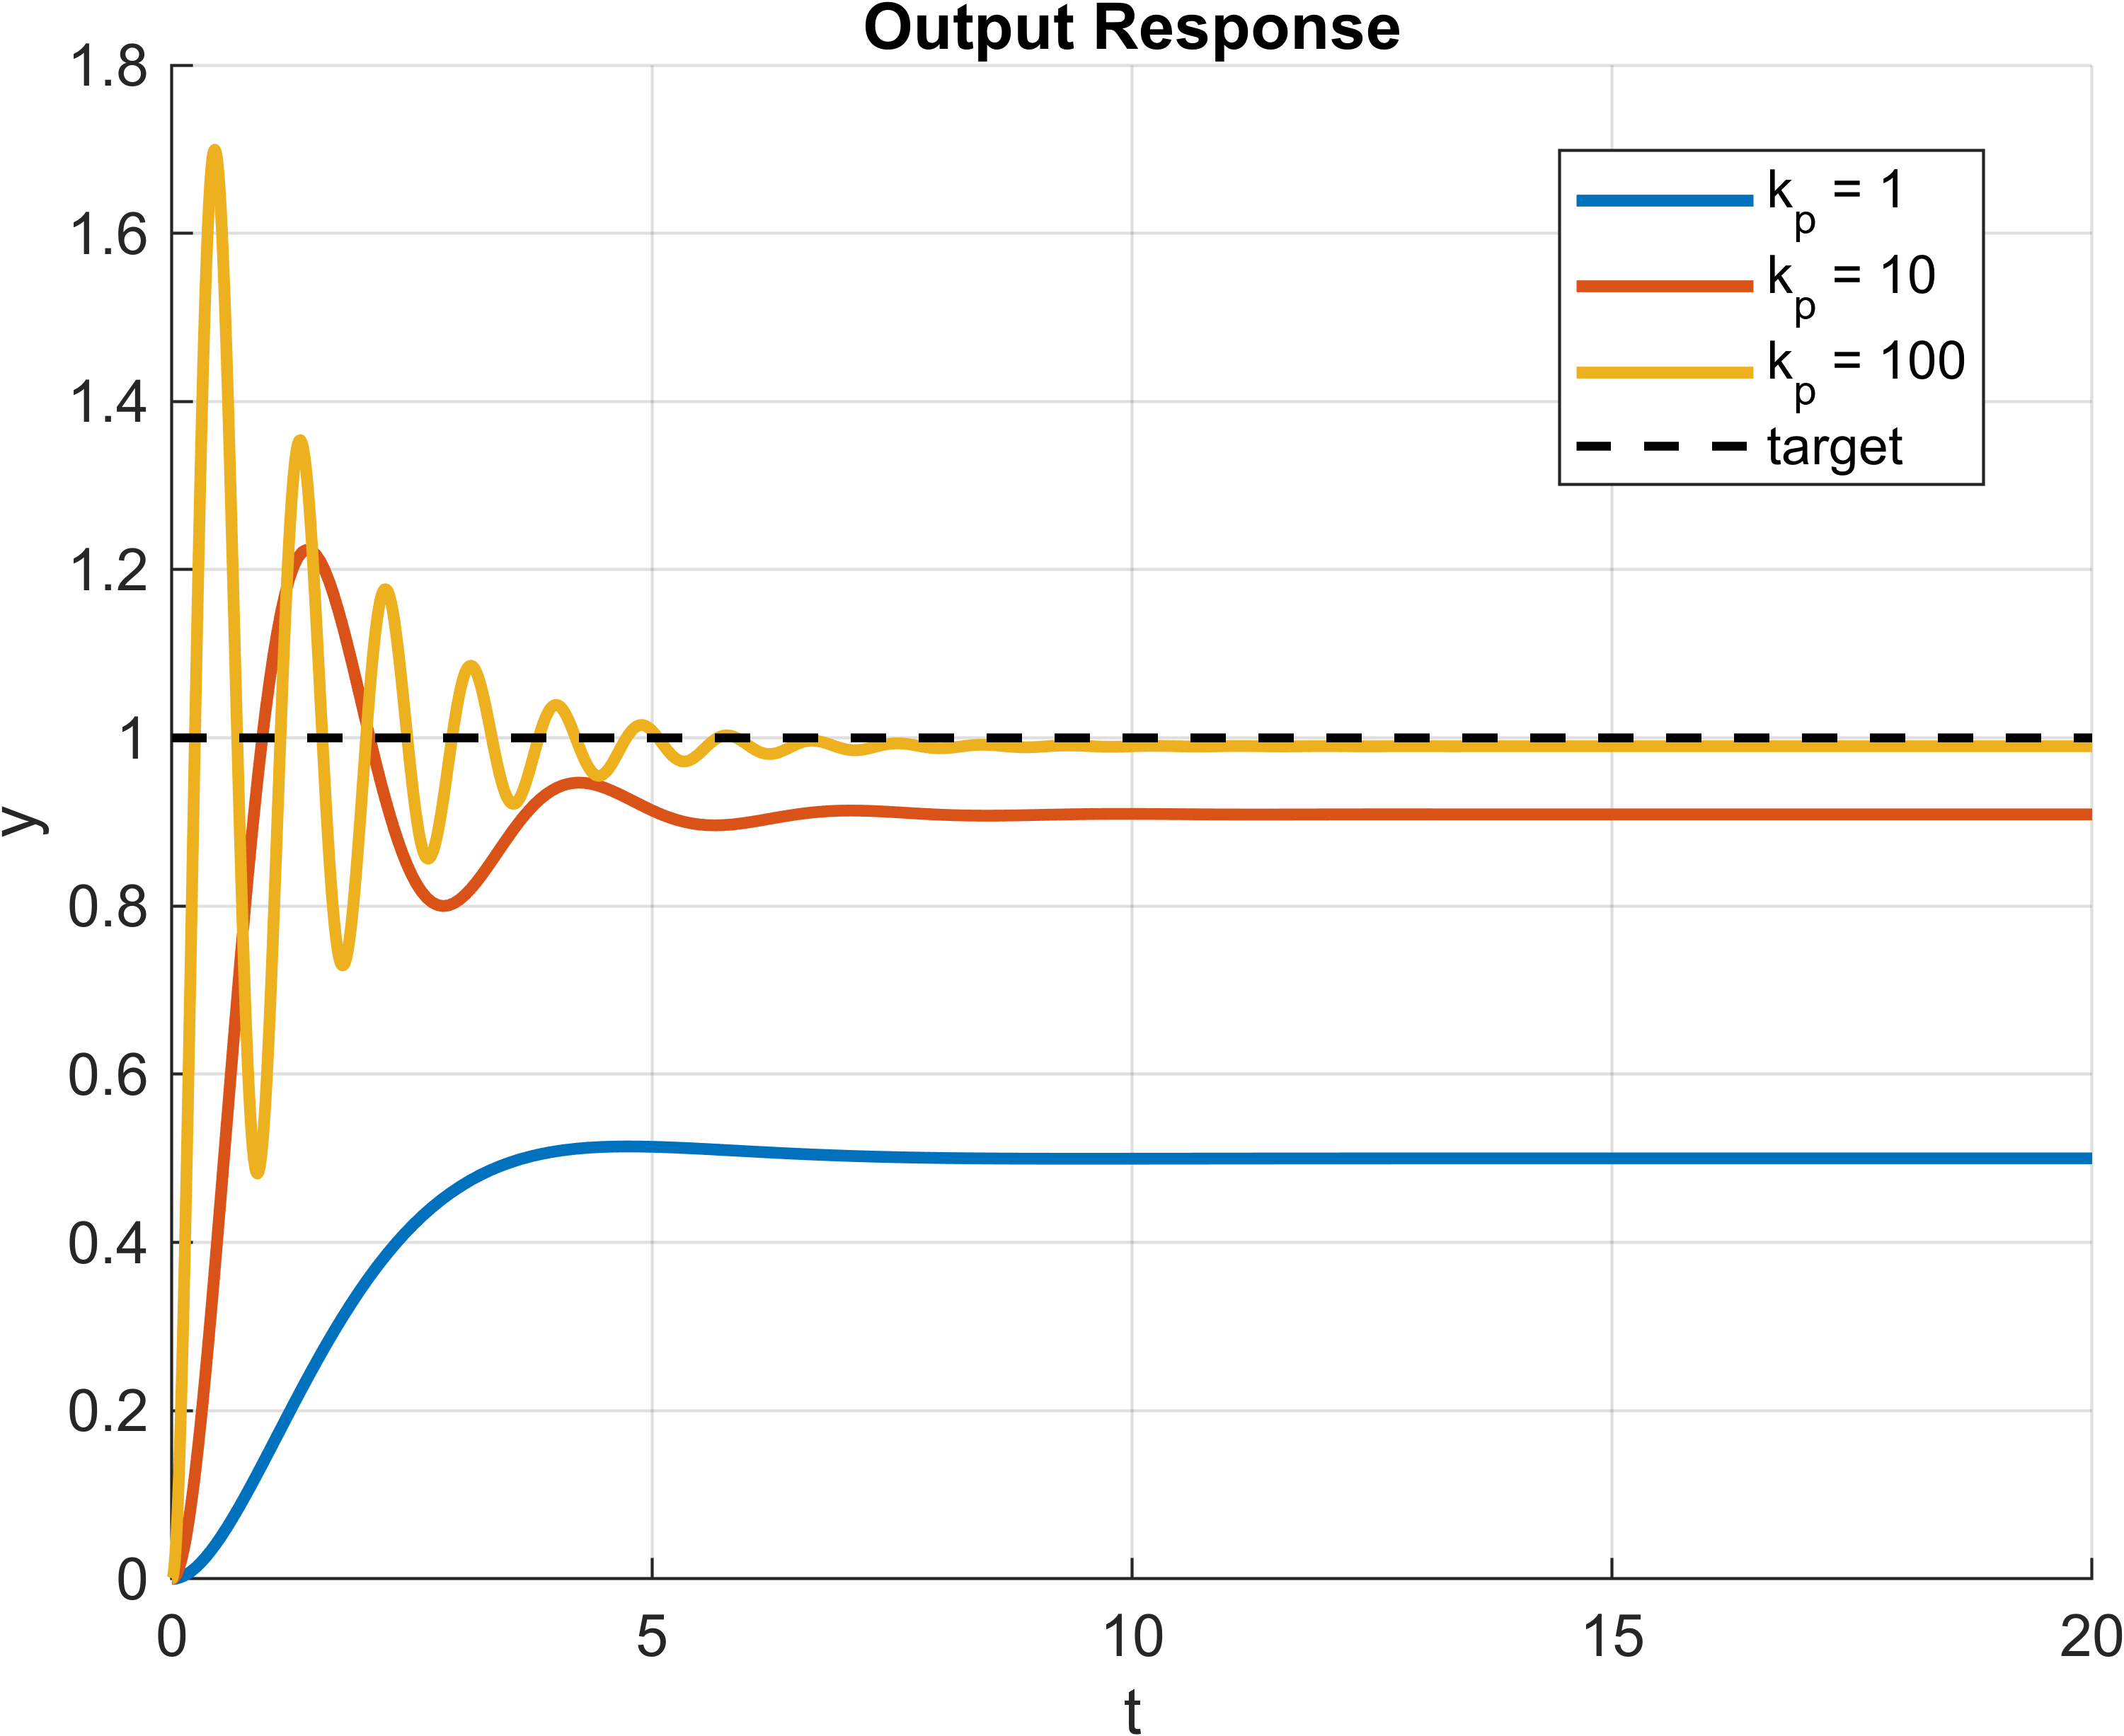
\includegraphics[width=1\textwidth, trim={1cm 0cm 1cm 0cm}]{../images/3_1.png}
    \end{minipage}
    \hfill
    \begin{minipage}{0.45\textwidth}
        \centering
        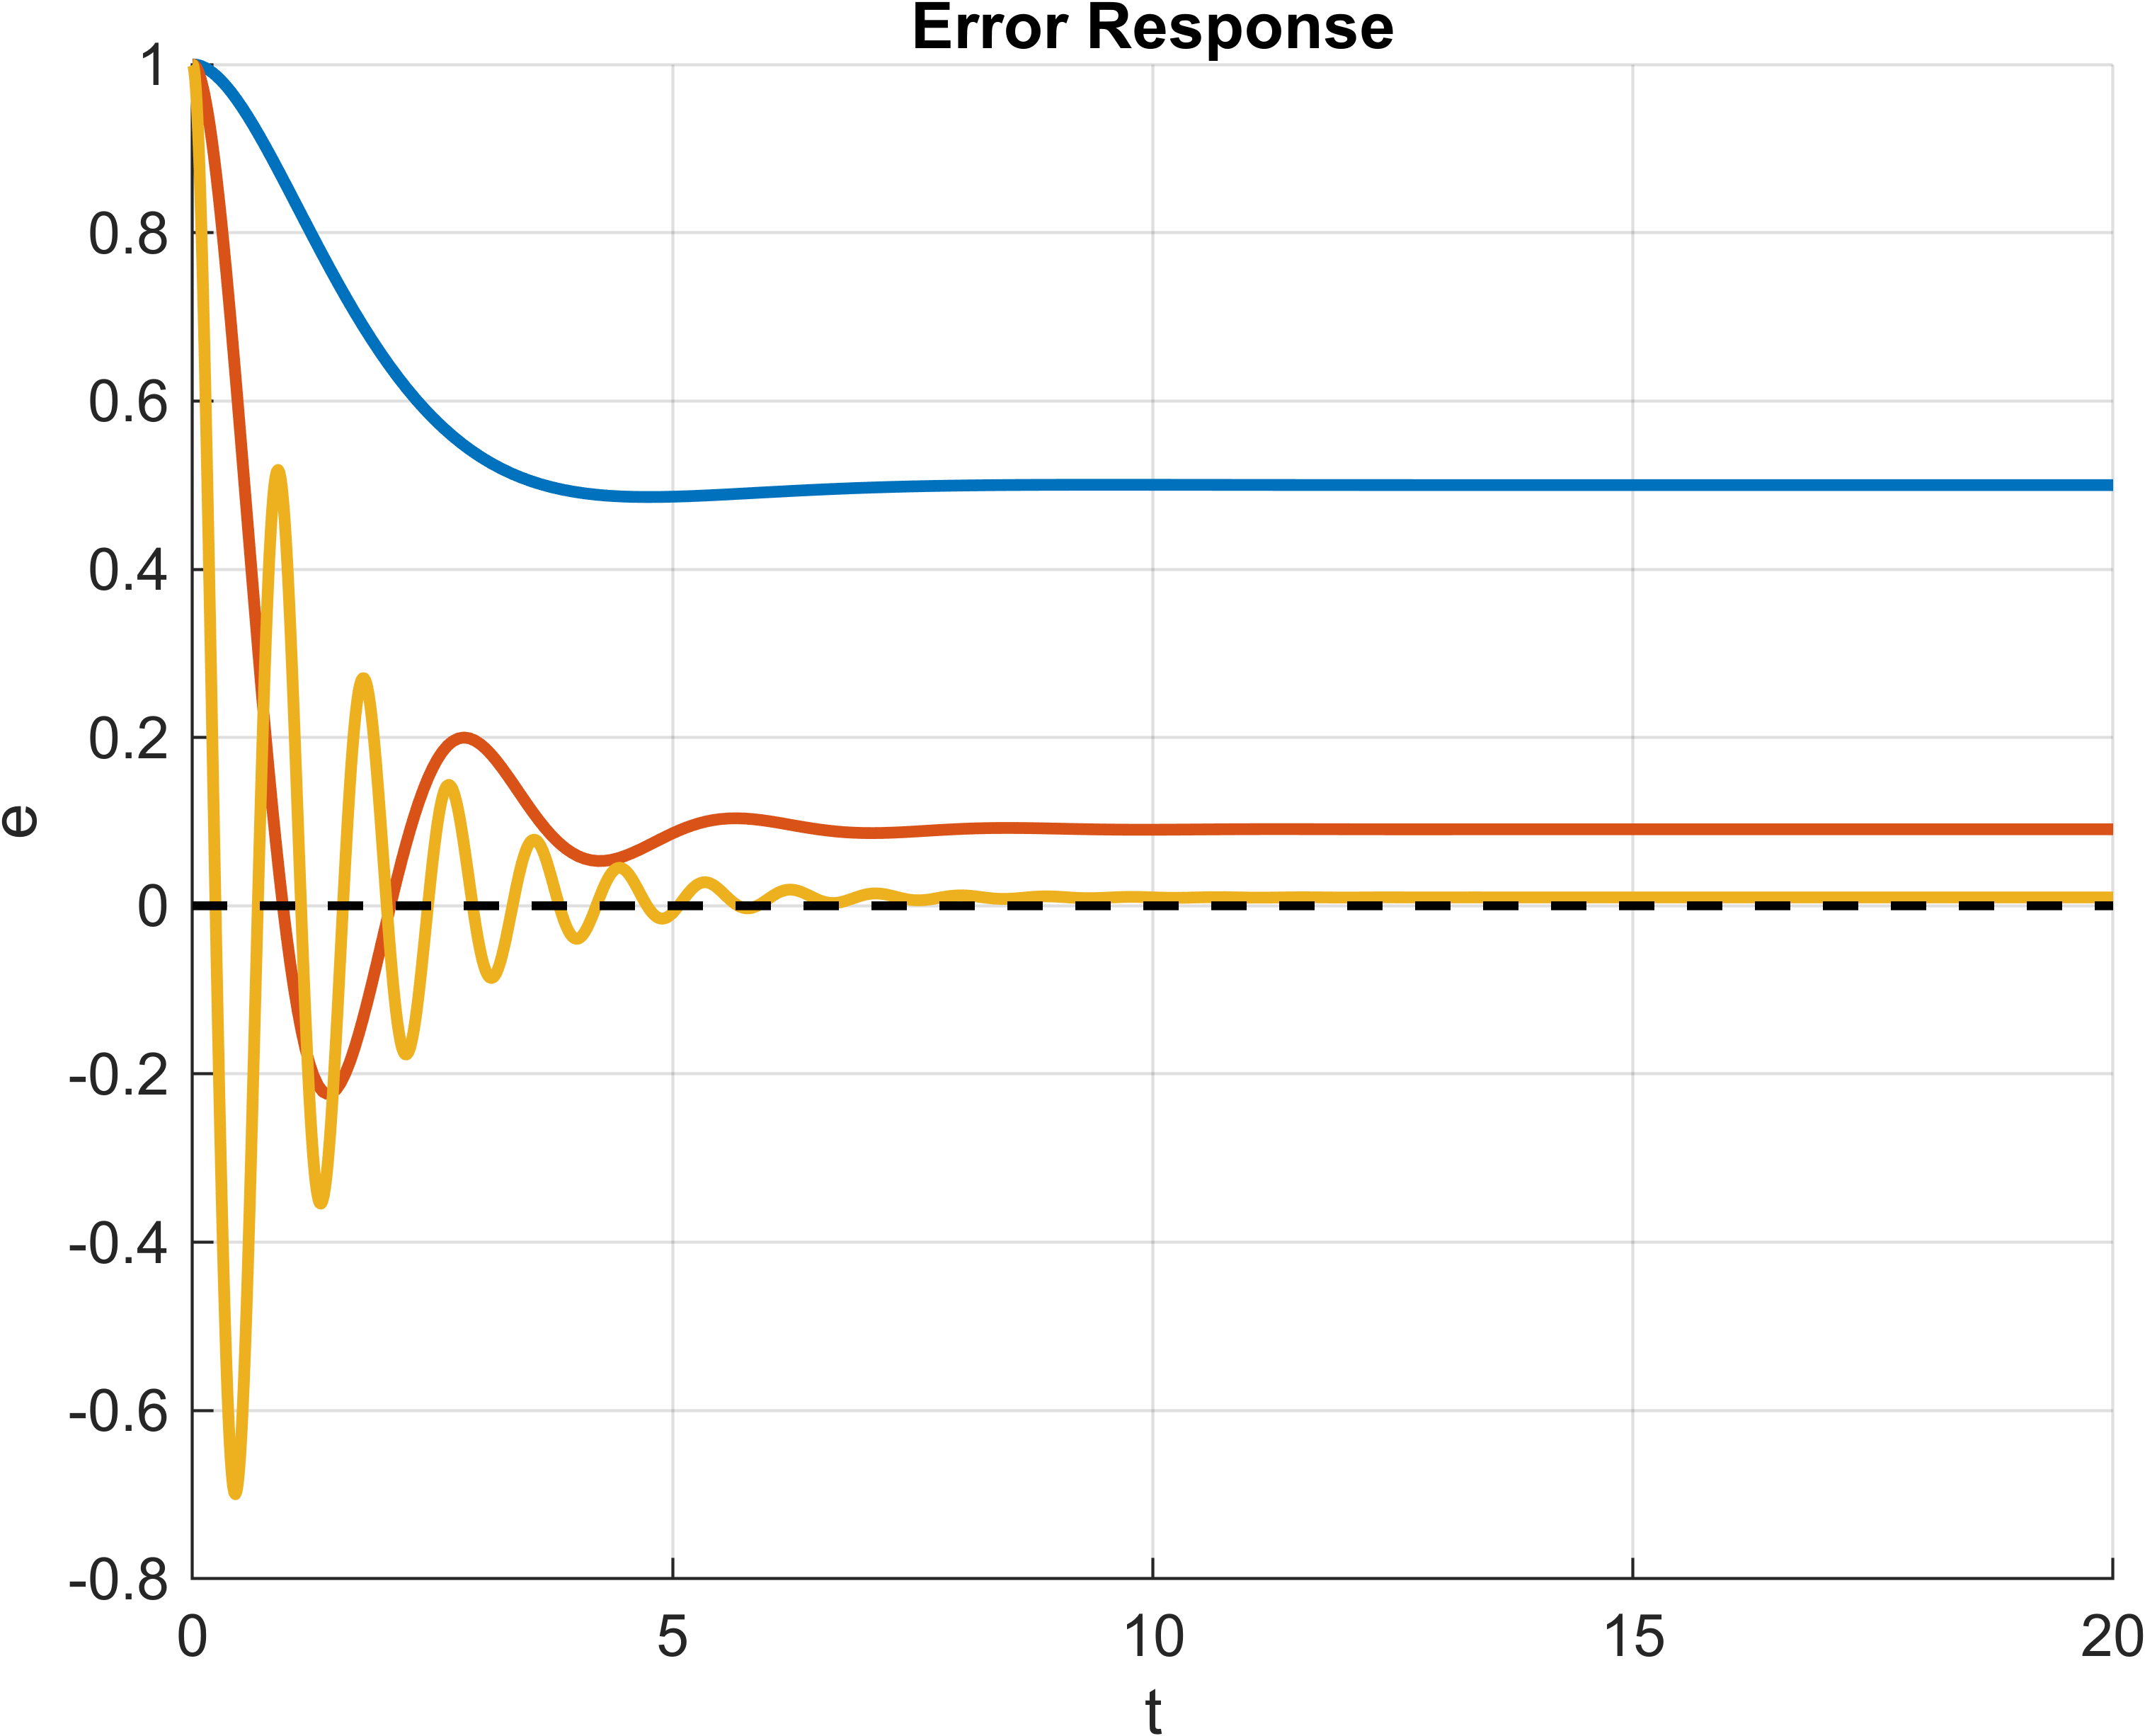
\includegraphics[width=1\textwidth, trim={1cm 0cm 1cm 0cm}]{../images/3_2.png}
    \end{minipage}
    \caption{Графики $y(t)$ и $e(t)$ при $g(t) = A$}
\end{figure}

Аналитически определим предельное значение ошибки $e$ для каждого значения $k_p$:
\[
W_{g\to e} = \frac{1}{1 + k_p W(s)} 
= \frac{1}{1 + k_p \frac{1}{2s^2 + 3s + 1}} 
= \frac{2s^2 + 3s + 1}{2s^2 + 3s + 1 + k_p}
\]
\[
e_{\text{уст}} = \lim_{t \to \infty} e(t) 
= \lim_{s \to 0} s E(s) 
= \lim_{s \to 0} s W_{g\to e} G(s) =
\]\[
= \lim_{s \to 0} s \frac{2s^2 + 3s + 1}{2s^2 + 3s + 1 + k_p} \frac{1}{s}
= \frac{1}{1 + k_p}
\]
\[
k_p = 1: \, e_{\text{уст}} = \frac{1}{2} = 0.5
\]
\[
k_p = 10: \, e_{\text{уст}} = \frac{1}{11} \approx 0.0909
\]
\[
k_p = 100: \, e_{\text{уст}} = \frac{1}{101} \approx 0.0099
\]

Как видно из графиков и аналитических расчетов, для стационарного режима
П-регулятор обеспечивает постоянную установившеюся ошибку. При увеличении
коэффициента $k_p$ ошибка уменьшается.
\newpage
\section{Режим движения с постоянной скоростью $g(t) = Vt$}
Выполним моделирование:
\begin{figure}[H]
    \centering
    \begin{minipage}{0.45\textwidth}
        \centering
        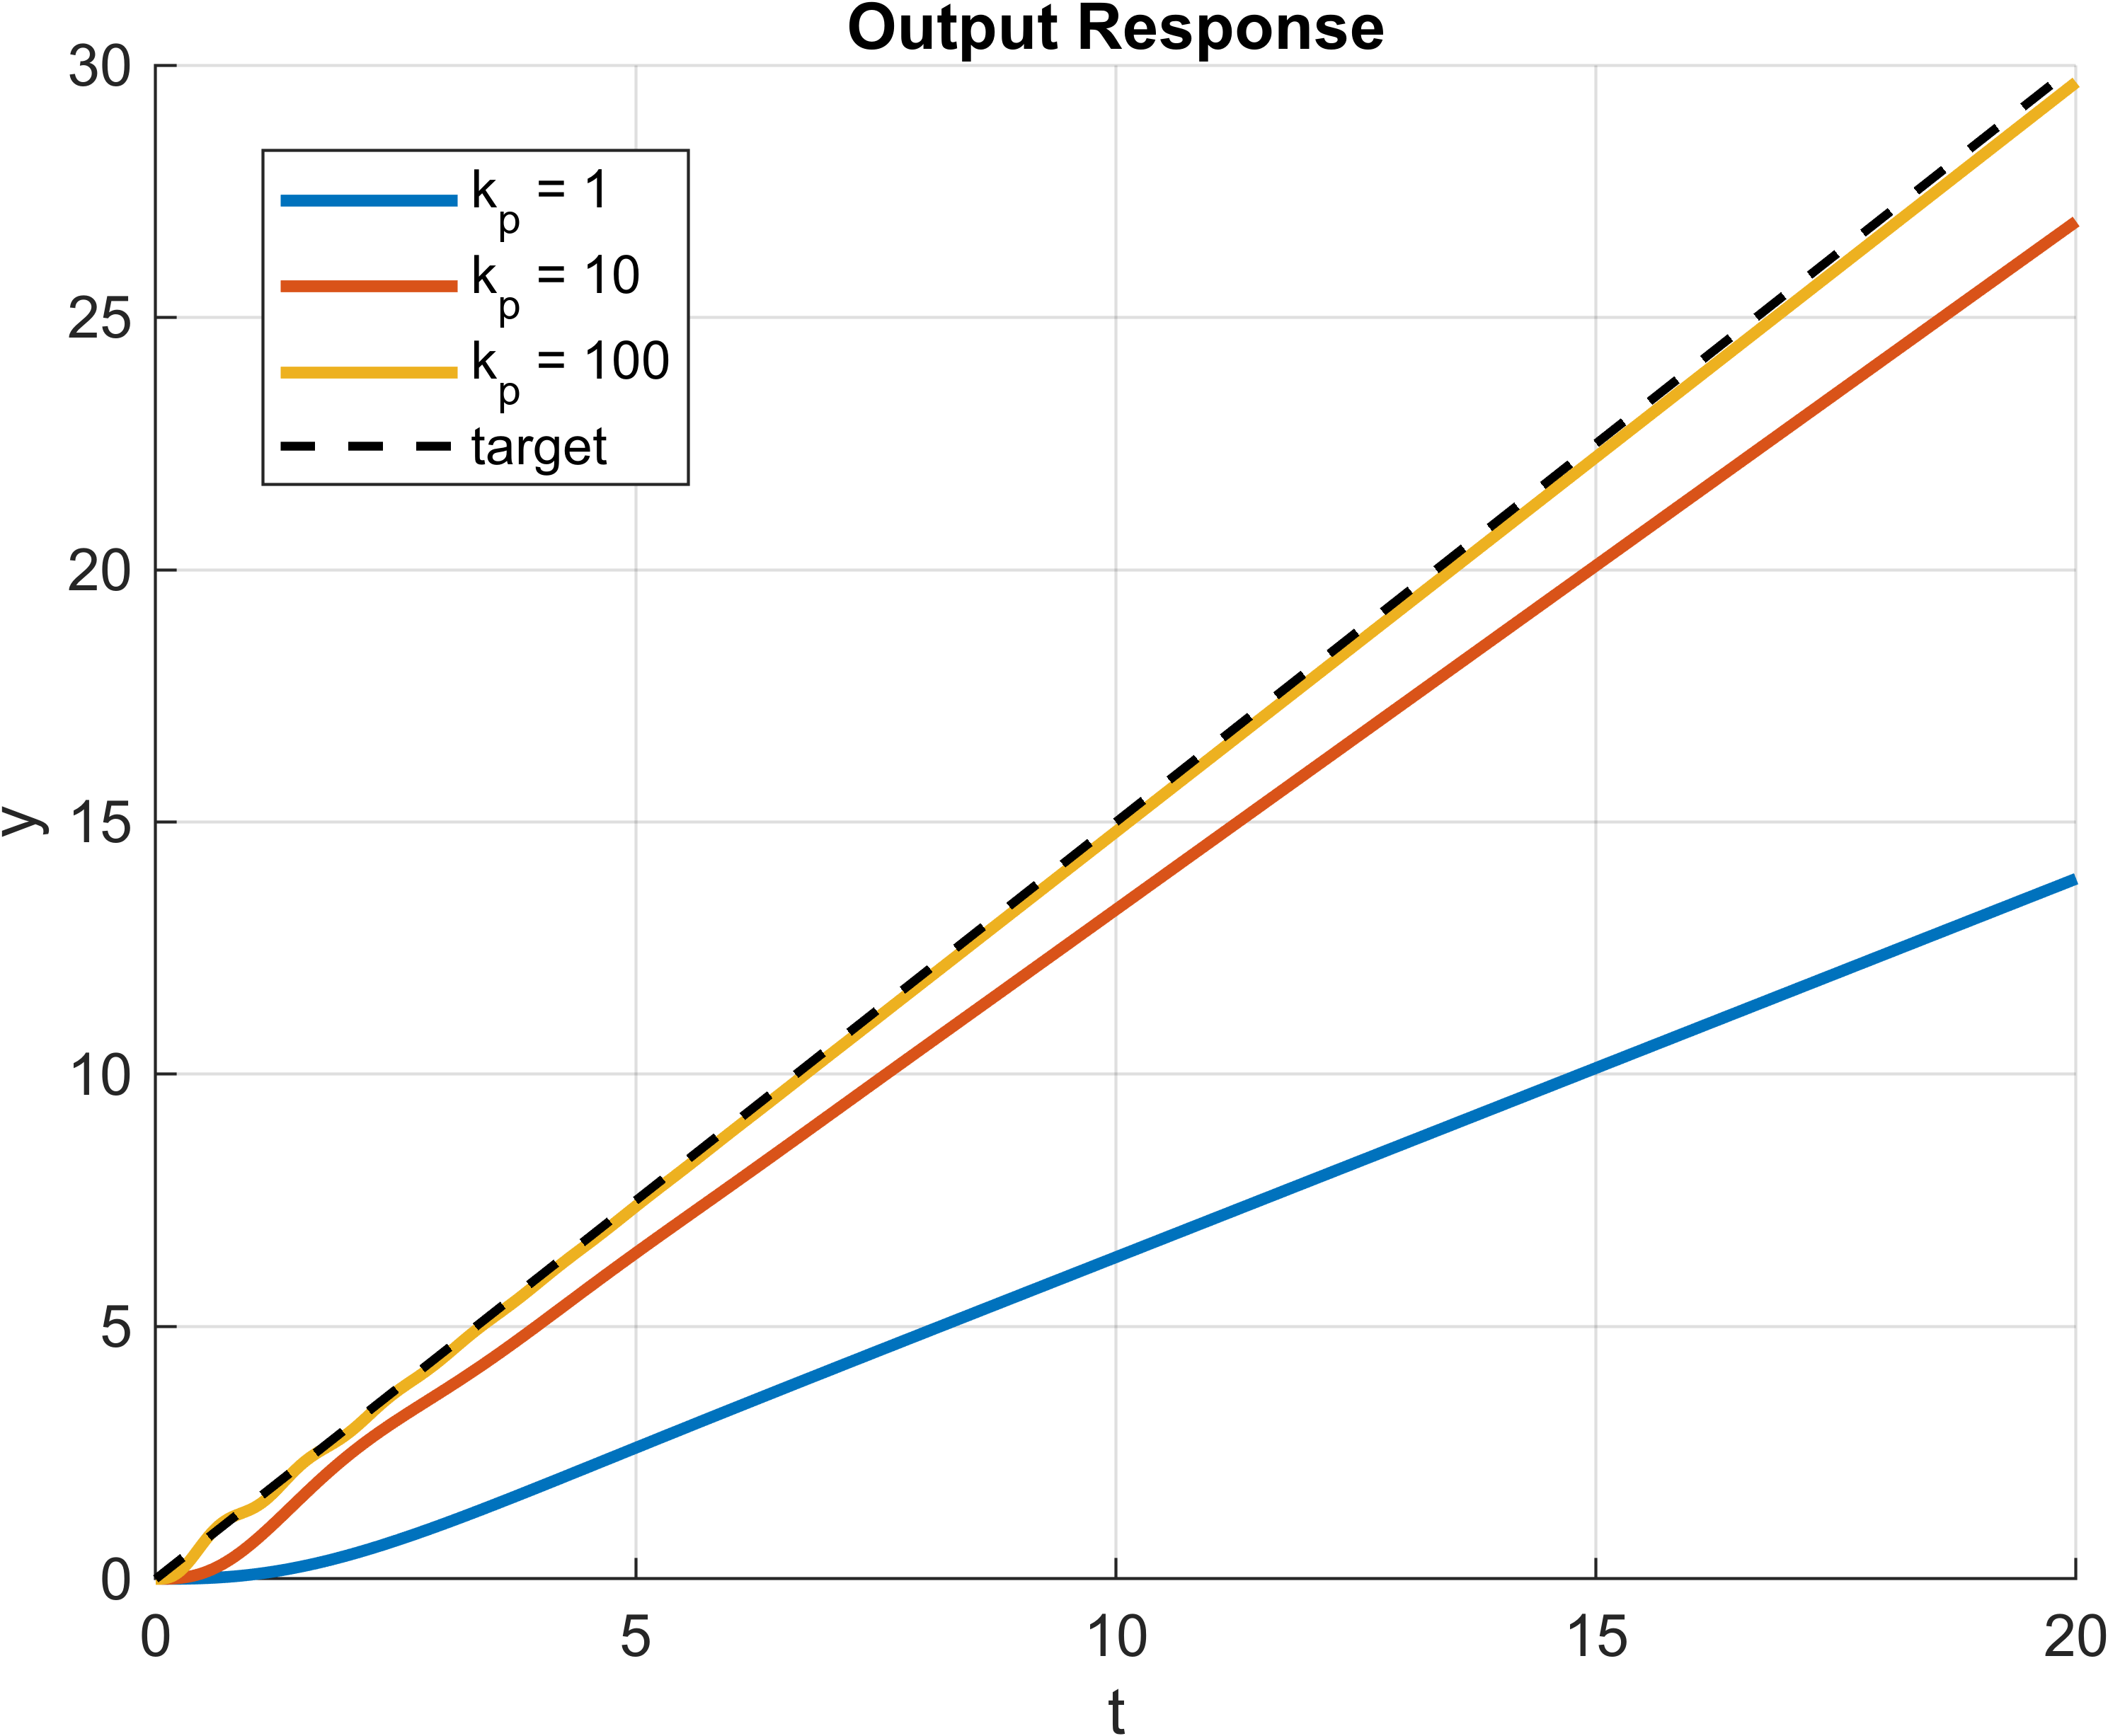
\includegraphics[width=1\textwidth, trim={1cm 0cm 1cm 0cm}]{../images/3_3.png}
    \end{minipage}
    \hfill
    \begin{minipage}{0.45\textwidth}
        \centering
        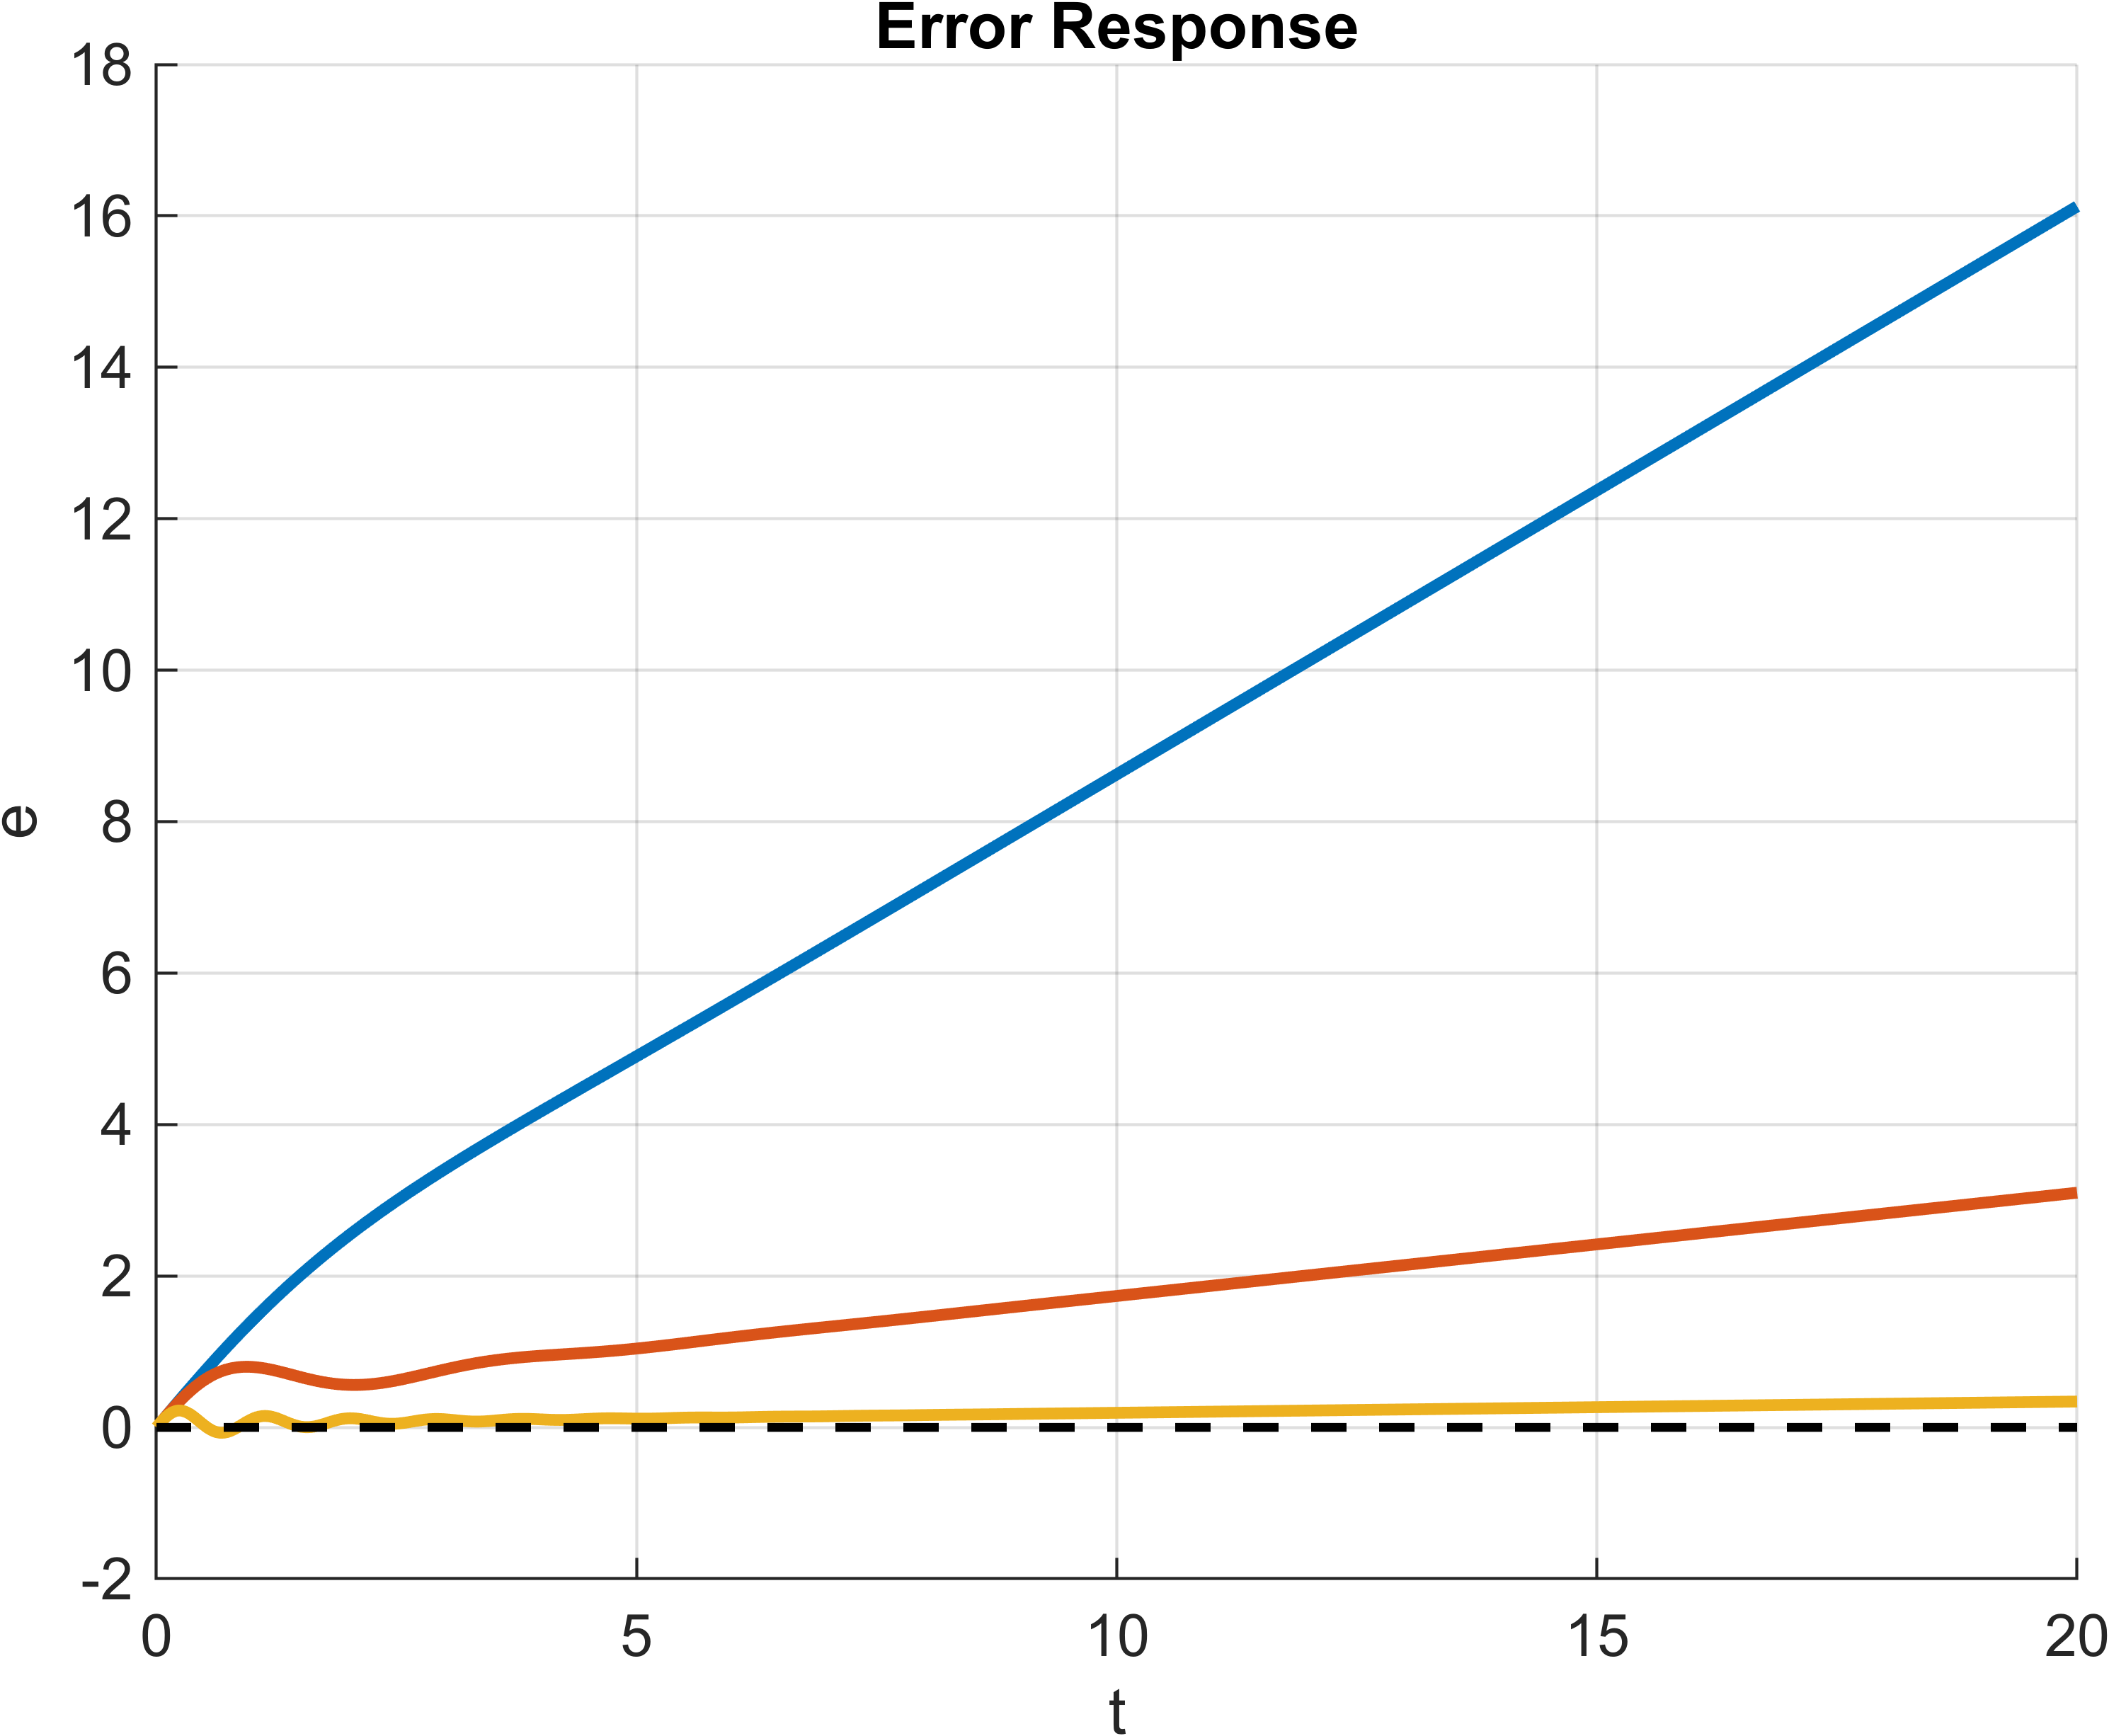
\includegraphics[width=1\textwidth, trim={1cm 0cm 1cm 0cm}]{../images/3_4.png}
    \end{minipage}
    \caption{Графики $y(t)$ и $e(t)$ при $g(t) = Vt$}
\end{figure}

Так как П-регулятор имеет нулевой порядок астатизма, 
то в режиме движения с постоянной скоростью $g(t) = Vt$
он не может обеспечить постоянную ошибку.
Она стремится к бесконечности, при увеличении 
коэффициента $k_p$ ошибка растет медленнее.
\endinput